\section{Iterative Architecture Evolution}

\subsection{Development Methodology}

The backend was developed using the Agile methodology, with each iteration spanning for a specific sprint. Each iteration was designed to produce a testable and potentially shippable increment of the backend. The allowed for regular feedback and continuous refinement of the architecture and features. Each iteration addressed a potential bottleneck of the system. Translation performance was manually tested using Postman\cite{postman2025} to analyse the most optimal design.

\subsection{Iteration 1: Baseline Sequential Processing}

\subsubsection{Implementation Approach:} Initial service logic was design to process each translation requests sequentially and converting data received from frontend to string arrays and submit it as a single request to LibreTranslate engine.

\begin{figure}[H]
    \centering
    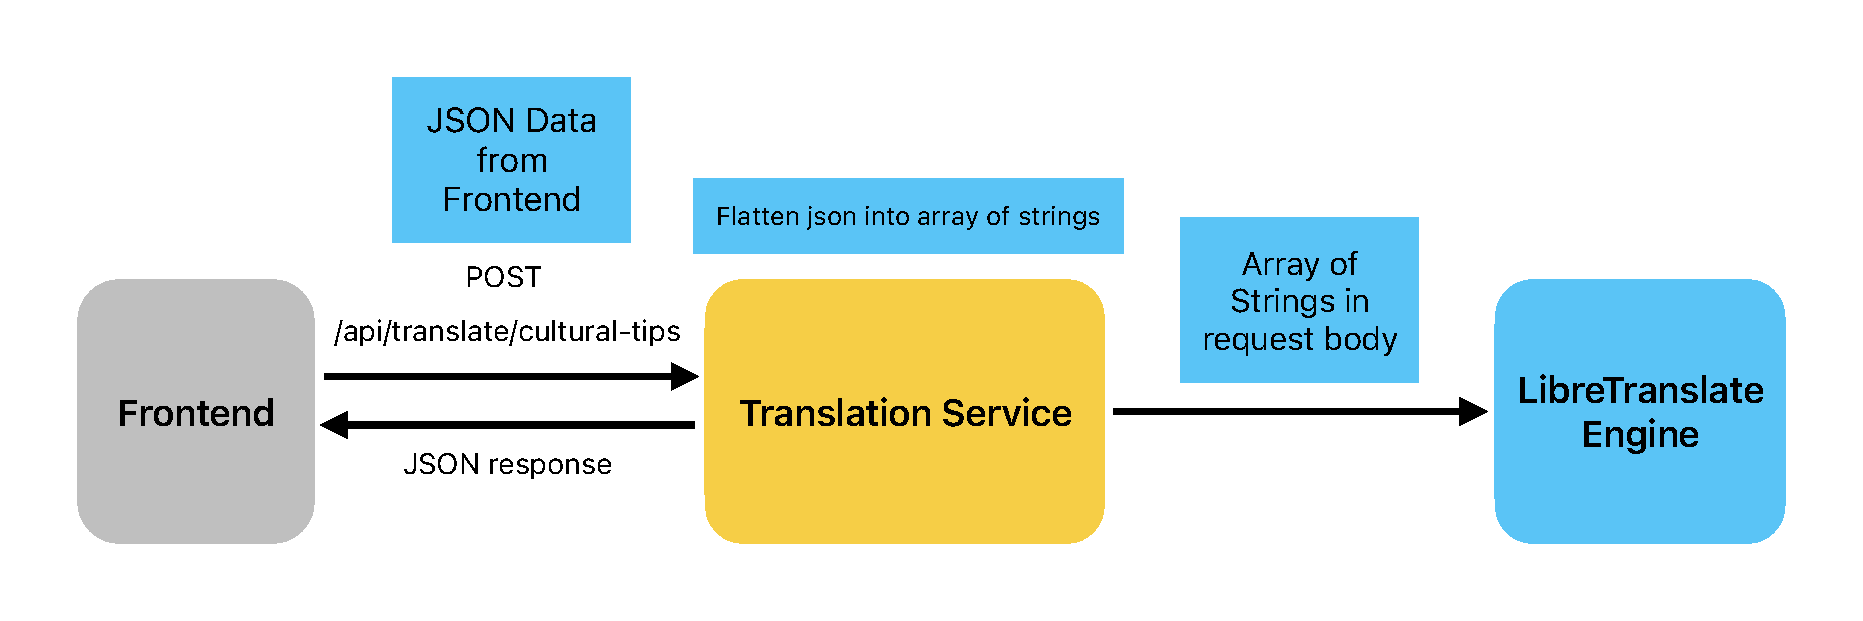
\includegraphics[width=1\linewidth]{chapter/05_implementation/backend/B_architectural_design/Backend_Initial_Concept.pdf}
    \caption{Initial iteration of backend service}
    \label{fig:backend_iteration_1}
\end{figure}

Initial manual performance tests done with the help of Postman Tool\cite{postman2025} established a baseline for the system's translation capabilities. The results showed an average response time of approximately 5.3 seconds (see response screenshot \ref{fig:intial_response_time}) for typical requests involving cultural tips data, which consisted of mulitple text segments. The largest segments being the transportation and payment information.

A bottleneck analysis of the baseline tests revealed that the performance contraint was not the LibreTranslate engine, but rather the translation service's sequential request orchestration logic. This approach failed to fully utilise the LibreTranslate's multi-threading capabilities, creating an artificial bottleneck which led to high response time. This finding was a key learning point, which validated that the initial architecture was not efficiently using the LibreTranslate engine. The results underscored the necessity of re-architecting an optimal solution to incorporate a parallel processing pattern\cite{kleppmann2017designing}. The refined architecture implements a "scatter-gather" approach which, instead of sending a single request with a large array of text, the translation service logic will divide the array into smaller chunks (the scatter phase) and dispatch multiple concurrent requests to the LibreTranslate engine. It then receives the requests from the LibreTranslate engine and aggregate them into a single response (the gather phase).

\subsection{Iteration 2: Parallel Processing Implementation}

The second implementation iteration was guided by the hypothesis that concurrent requests from translation service to LibreTranslate engine would reduce the overall system response time proportionally to the number of parallel requests sent to the LibreTranslate engine. A concurrency level of four was chosen to align with the LibreTranslate's default thread count configuration\cite{libretranslate_docs_installation}. A key technical challenge was partitioning the variable length sentences into four equally balanced batches. This is to ensure each response time from LibreTranslate engine is close enough to reduce threads from waiting in the translation service. To achieve this, greedy algorithm was used to solve the load balancing problem of distributing the sentences into batches. A greedy algorithm is an algorithmic paradigm that makes a locally optimal choice at each store with the hope of finding a global optimum solution\cite{geeksforgeeks_greedy}\cite{kleinberg2006algorithm}\cite{wiki:greedy_partitioning}. In our specific implementation, the algorithm's goal is to partition a list of sentences into a fixed number of batches so that the total character count of each batch is roughly equal. The 
algorithm works by first sorting the sentences by length in descending order and then iteratively making the "greedy" choice of assigning it to the batch with lowest cumulative character count and repeating the process until all sentences are distributed into batches.

Another primary challenge in implementing parallelisation was the task of sentence boundary disambiguation, that is the process of accurately splitting a large text into individual sentences without losing semantic context. Initial approach of splitting large text based on punctuation using regular expression deemed to be unreliable. It fails to correctly interpret complex sentences containing abbreviations, quotations, or non-terminal punctuations, which could degrade the quality of translation output\cite{walker_et_al_2001}.

To mitigate this, we integrated the Apache OpenNLP library, a standard toolkit for natural language processing (NLP). OpenNLP's open-source pre-trained sentence splitting model\cite{apache_opennlp_models} is trained on large corpora to identify sentence boundaries with contextual awareness, significantly outperforming regex-based approaches. The library achieved an accuracy rate of approximately 93\% for sentence boundary detection, which deemed acceptable for our application context\cite{apache_opennlp_manual_2_3_2}.

\begin{figure}[H]
    \centering
    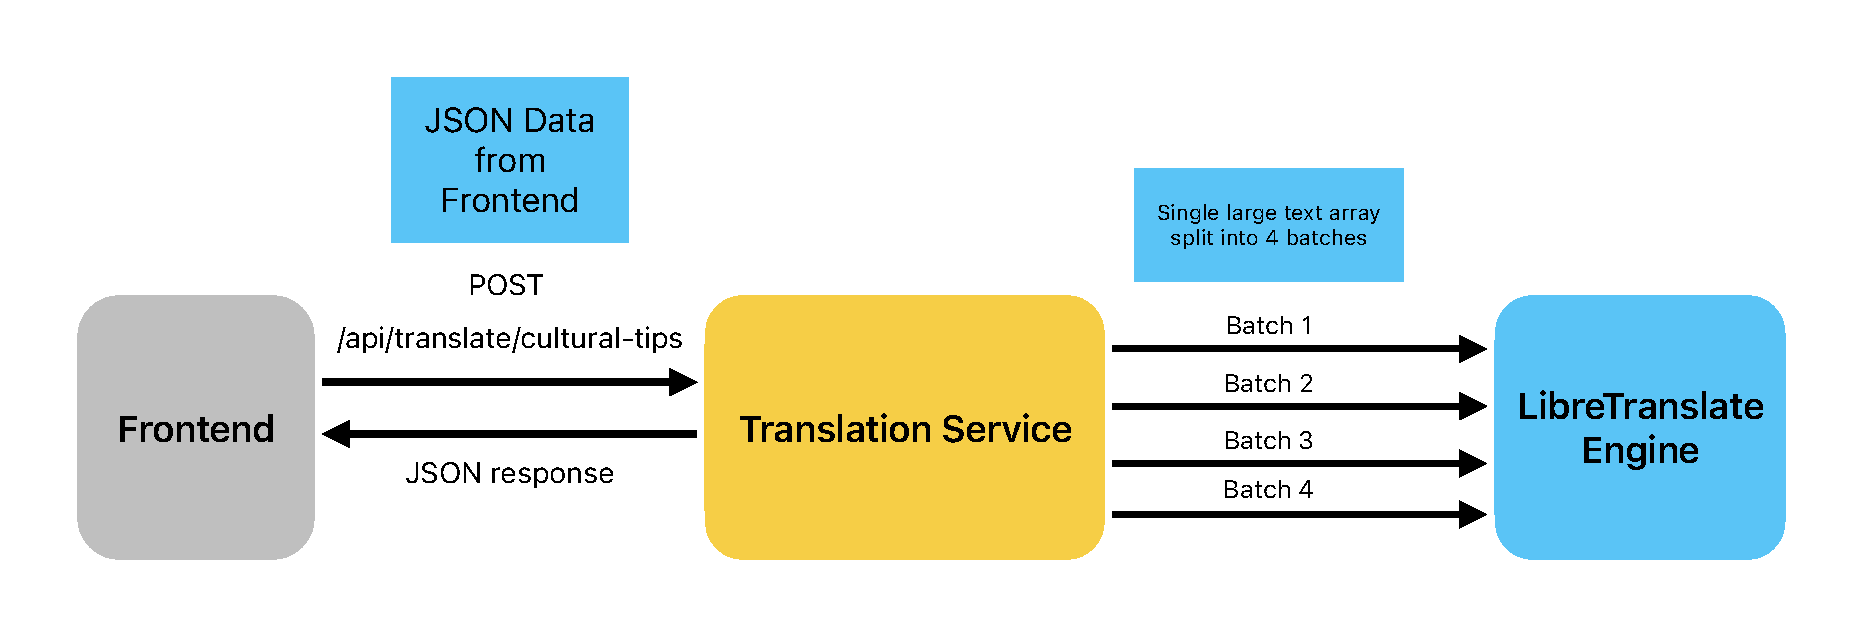
\includegraphics[width=1\linewidth]{chapter/05_implementation/backend/B_architectural_design/Backend_Iteration_2.pdf}
    \caption{Second iteration of backend service}
    \label{fig:backend_iteration_2}
\end{figure}

Manual testing of the new implementation approach showed a 20\% reduction in average response time (reduction from approximately 5.3 seconds to 4.3 seconds, see response screenshot \ref{fig:20_reduction_response}) compared to baseline. However, this was a minimal performance gain that did not align with the expected improvement of theoretical 4x improvement from four-way parallelisation. On further analysis the key issue turned out it be that the LibreTranslate thread pool only affects the web server thread pool and not the underlying CTranslate2 translation engine used in the backend. LibreTranslate's backend engine CTranslate2 Translate has its own internal threading contraints that limits full utilisation of multiple cores\cite{euno2023unable}. While the web server can handle 4 requests concurrently, but the actual translation is still largely sequential within the CTranslate2 engine as noted in CTranslate2 github discussions\cite{hobodrifterdavid}. This discovery revealed that the performance bottleneck had shifted from request serialisation to LibreTranslate engine's capacity limitation, indicating that horizontal scaling through distributed processing architecture would be required. The subsequent architectural iteration must therefore focus on distributing the translation load across multiple LibreTranslate instances to circumvent the natural processing limits of the single instance.

\subsection{Iteration 3: Horizontal Scaling with Service Discovery}

\subsubsection{Architectural Decision and Challenges:} Based on the insights from the previous iteration, the architectural strategy pivoted from vertical optimisation to horizontal scaling. The goal was to distribute the translation load from the frontend equally across multiple LibreTranslate instances. Initial implementation attempt to use kubernetes, which "is a portable, extensible, open source platform for managing containerized workloads and services" \cite{kubernetes_overview}\cite{burns2022kubernetes}. Kubernetes manages the containerised application inside a pod, "Pods are the smallest deployable units of computing that you can create and manage in kubernetes"\cite{kubernetes_pods}. But the kubernates-native load balancing revealed some challenges. The REST client's connection pooling mechanism was limiting the Kubernetes cluster's inbuilt load balancer\cite{kubernetes_services_networking}\cite{redhat_kubernetes_cluster}, which was causing numerous consecutive requests to the same instance despite the availability of other instances in the cluster\cite{expedia_load_distribution}\cite{pubsapient_uneven_distribution}. 
The kubernetes cluster was configured for horizontal pod autoscaling, "horizontal scaling means that the response to increased load is to deploy more Pods." \cite{kubernetes_horizontal_pod_autoscaling}.
This resulted in ineffective load distribution and premature CPU-based auto-scaling triggers, where new instances were provisioned but did not receive traffic.

\subsubsection{Solution Architecture:}
\begin{figure}[H]
    \centering
    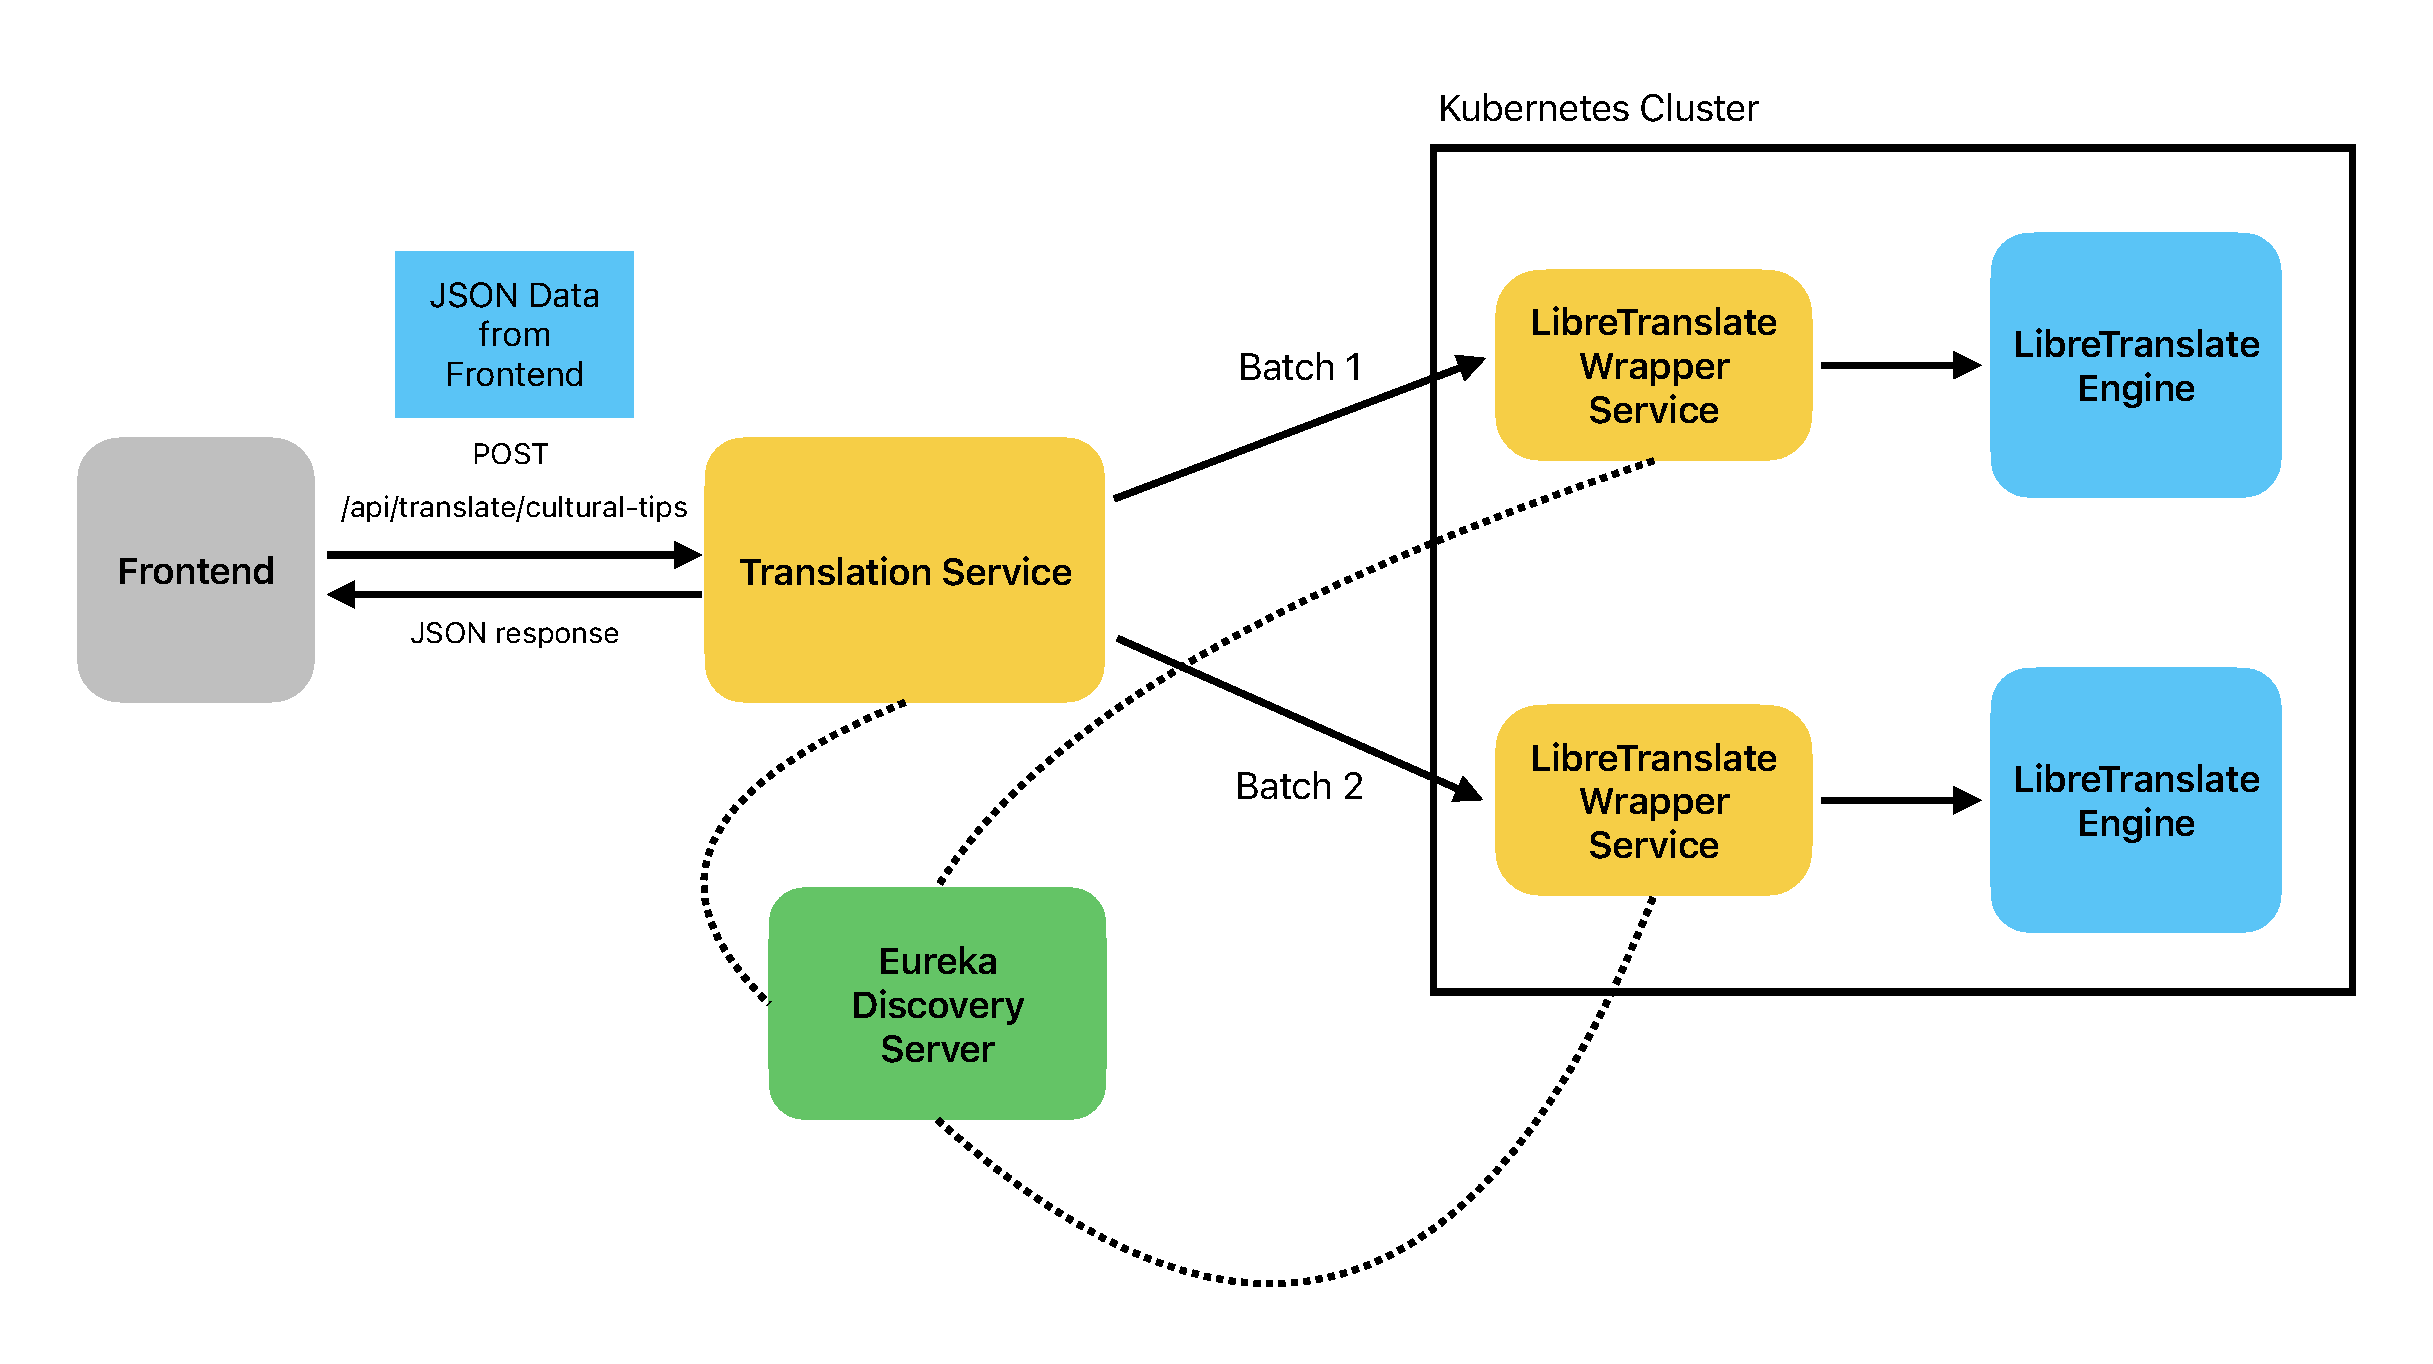
\includegraphics[width=1\linewidth]{chapter/05_implementation/backend/B_architectural_design/Backend_Iteration_3.pdf}
    \caption{Third iteration of backend service}
    \label{fig:backend_iteration_3}
\end{figure}

To overcome these challenges, the architecture was enhanced with an application-layer service discovery pattern, for which we selected Spring Cloud, this is due to our existing spring framework integration which provides seamless integration of additional tools required to extend the backend's functionality. "Spring Cloud provides tools for developers to quickly build some of the common patterns in distributed systems"\cite{spring_cloud}. Spring cloud provides Spring Cloud Netflix Eureka which is a "Netflix OSS integrations for Spring Boot apps through autoconfiguration and binding to the Spring Environment and other Spring programming model idioms"\cite{spring_cloud_netflix}\cite{carnell2021spring}\cite{netflix_eureka}. Eureka provides a more controlled load distribution mechanism, allowing client to be aware of all the available service instances. This enables fine-grained control over request routing, ensuring even distribution of requests across all available LibreTranslate instances and prevent the connection pooling issue.

To integrate LibreTranslate containers, there was a need for a wrapper service that would register with the Eureka server. This was needed as LibreTranslate engine is not based on java spring framework. The lightweight wrapper service was coupled in a 1:1 ratio with LibreTranslate engine, acting as an adapter. Its sole responsibility is to register with Eureka server and send requests to LibreTranslate engine. This pattern enabled the LibreTranslate engine to be discoverable within the microservices ecosystem and specially to the translation service from which the requests would be consumed. The wrapper service along with LibreTranslate engine would be deployed in a single container and as a single service unit, this would enable kubernetes to auto-scale based on the container's CPU utilisation and spin up more instances based on a threshold of 60\% container load.

This horizontally-scaled architecture help in keeping linear performance during high user loads. The throughput increased proportionally with the number of active LibreTranslate instances. Furthermore, the dynamic scaling policies optimised the resource utilisation, ensuring cost efficiency by only provisioning instances as required by the load. The critical success factor of this iteration was the implementation of the service discovery pattern that enabled scaling based on user load. Even though per user response time was not reduced, but the system ensured that the response time does not increase proportionally for the user load by sending multiple user requests to only on LibreTranslate engine.

\subsection{Iteration 4: Database Integration as a Persistent cache}

\subsubsection{Problem Identification:} 
Until the previous architecture iteration, it was the frontend's responsibility to get the cultural tips data from the AI agent and then send the data for translation to the backend's translation service. Manual analysis of the system under typical usage patterns revealed a significant performance and cost inefficiencies. Each user visiting the platform would trigger AI agent for cultural tips data, this resulted in recurring AI API costs and redundant translation processing for frequently request city data, causing unnecessary computational overhead for content. We identified that the city data like etiquettes, transportation, payment methods does not frequently change on every request, the data is usually constant for a long period of time\cite{govuk2020bus}\cite{bagheri2023global}\cite{zhang2021urban}\cite{tussey2025principles}.

\subsubsection{Solution Architecture and Implementation}

To address this, a persistent caching strategy using a relational database was implemented. We treated database as a durable cache to store both the English content and its translations. The database schema is designed to store city data with a 30-day refresh cycle. 

A new API endpoint (/api/v2/tips) was introduced in the translation service, keeping backward compatibility with the old api endpoint. The enhanced request handling workflow is as follows:
\begin{enumerate}
    \item For a requested city and language, the system performs a database query for existing data.
    \item If the database entry is not available or expired (a cache miss), then it is checked for English version of the content.
    \item If English version of the data is valid then we process the data for translation, otherwise AI Agent is invoked for fresh data and stored as the base record to support future translation needs.
    \item Translations are performed once per language and persistently cached for reuse.
    \item For cache hits, the system response directly from the database, bypassing costly and redundant translation and AI inference processes.
\end{enumerate}

\begin{figure}[H]
    \centering
    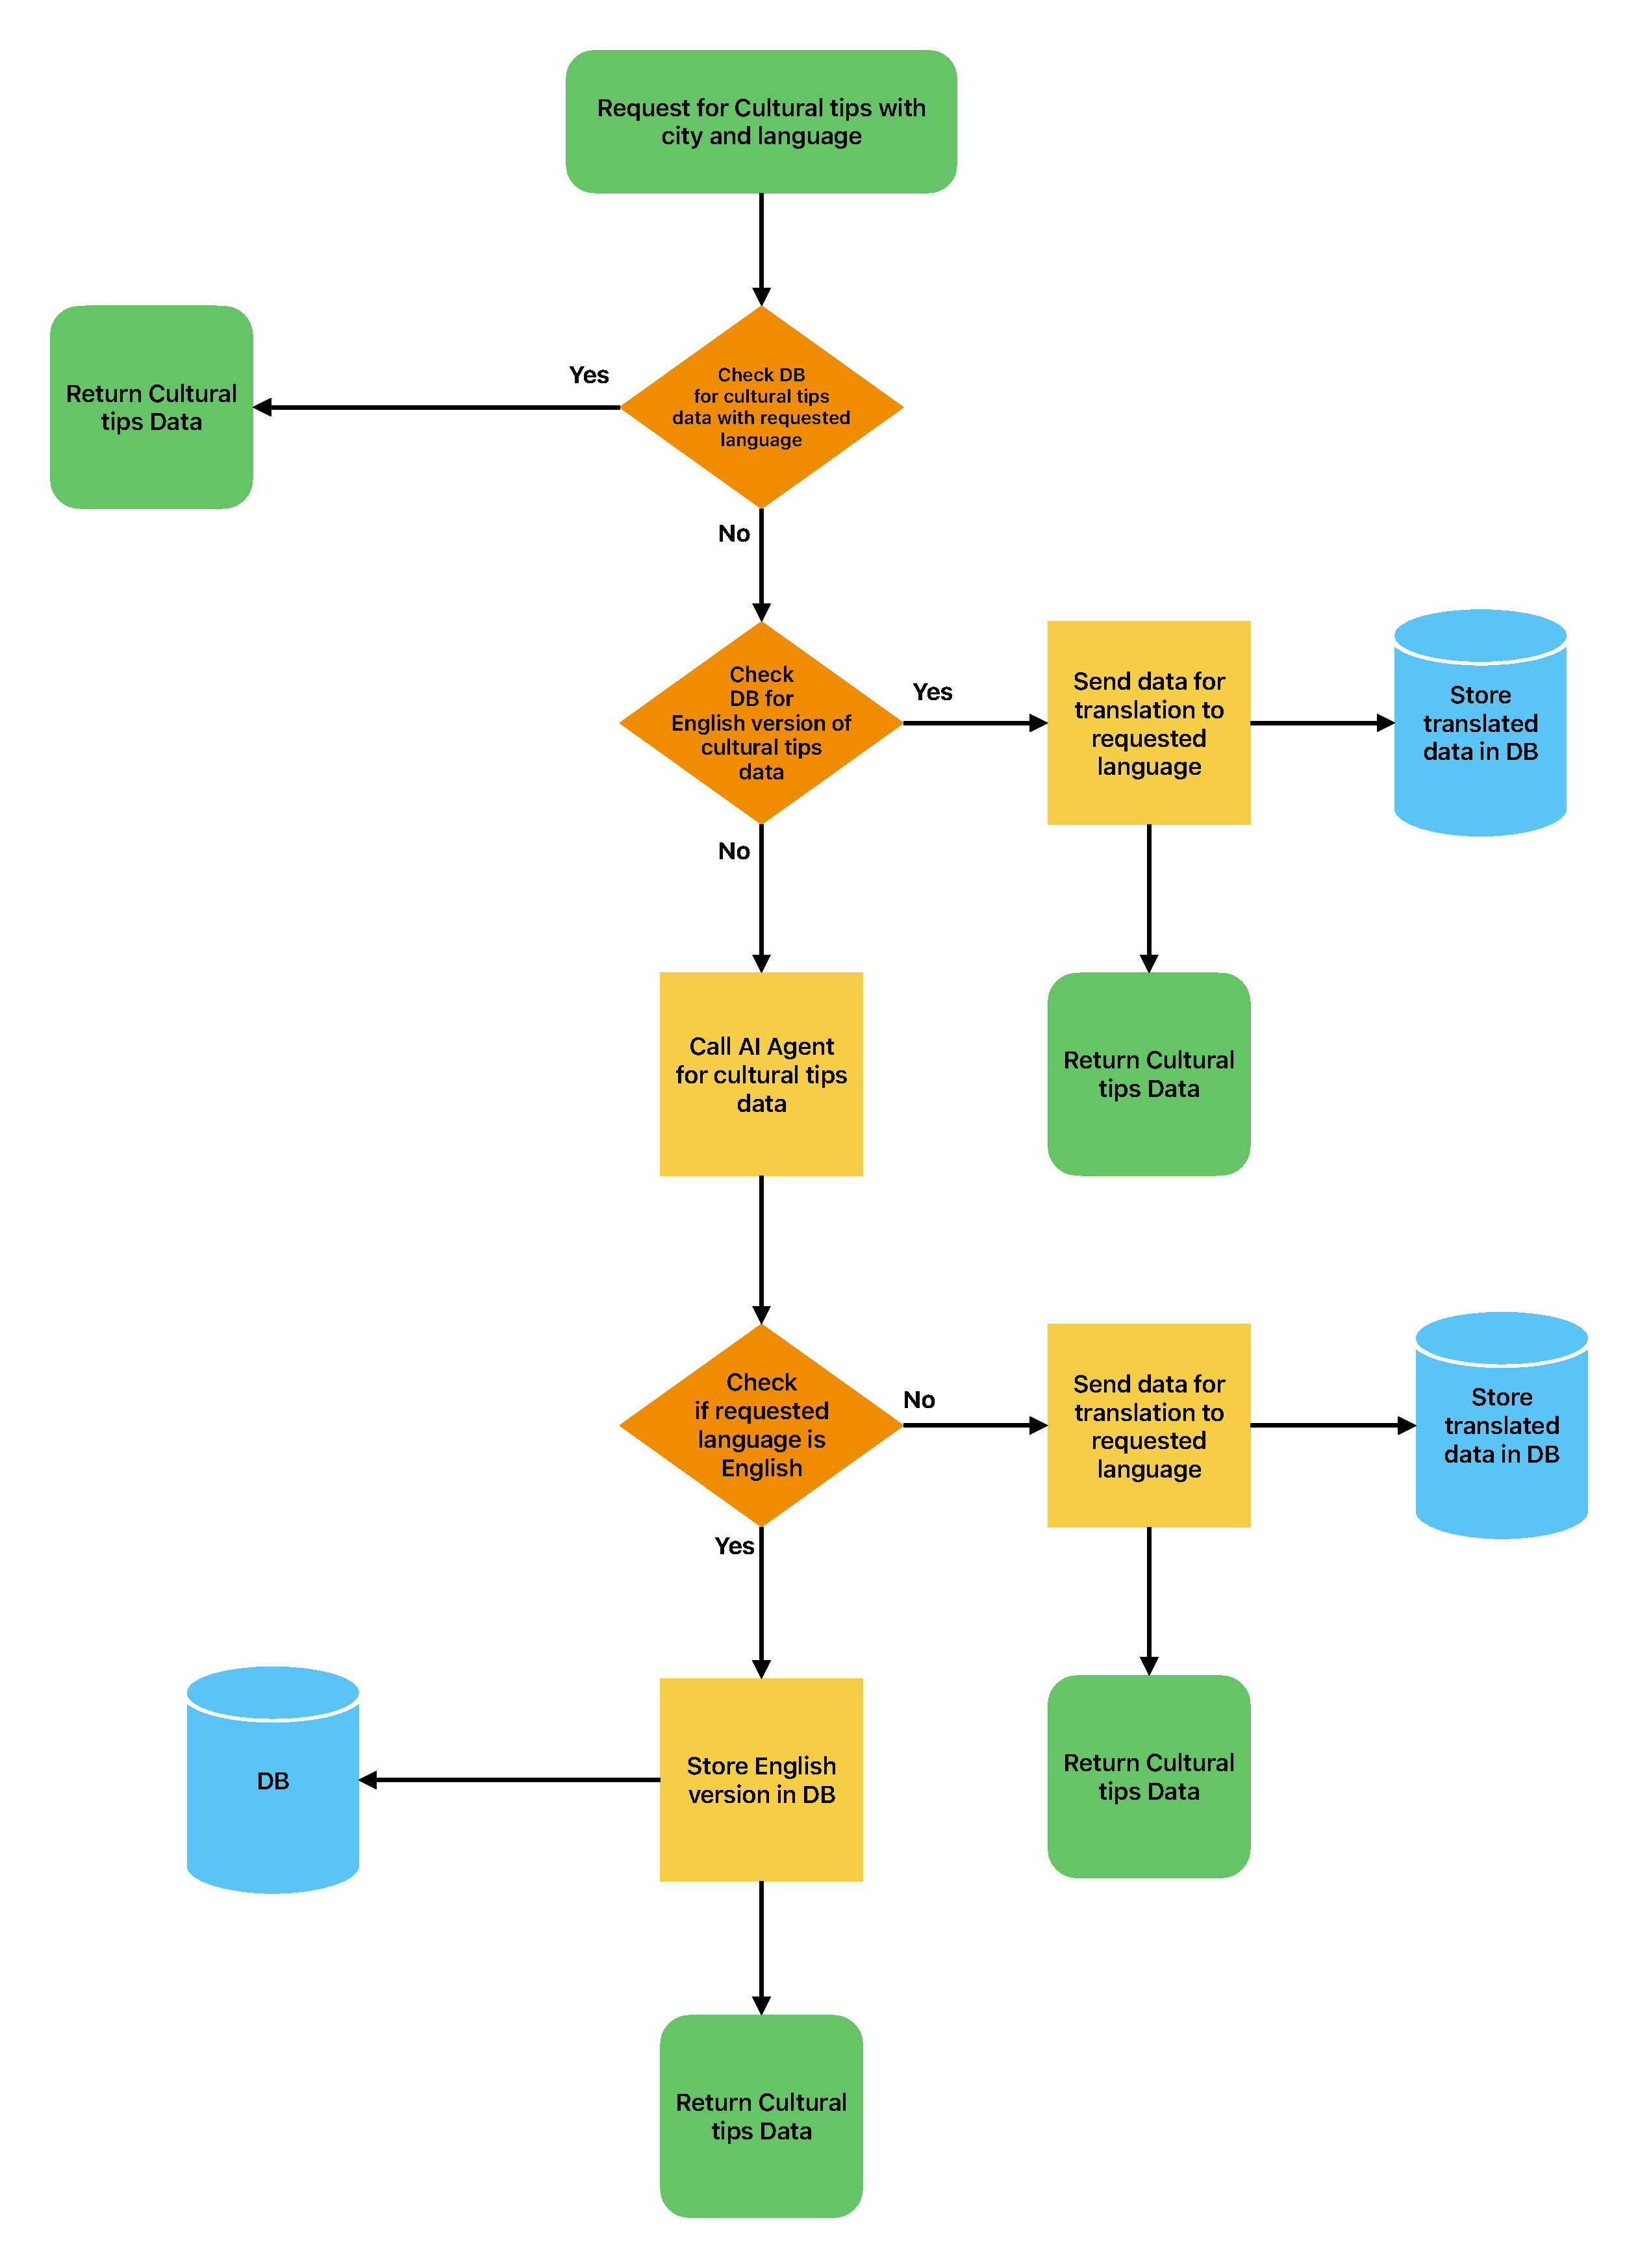
\includegraphics[width=1\linewidth]{chapter/05_implementation/backend/B_architectural_design/Business_Logic_Flow.pdf}
    \caption{Final business logic flow}
    \label{fig:backend_business_logic _flow}
\end{figure}



\begin{figure}[H]
    \centering
    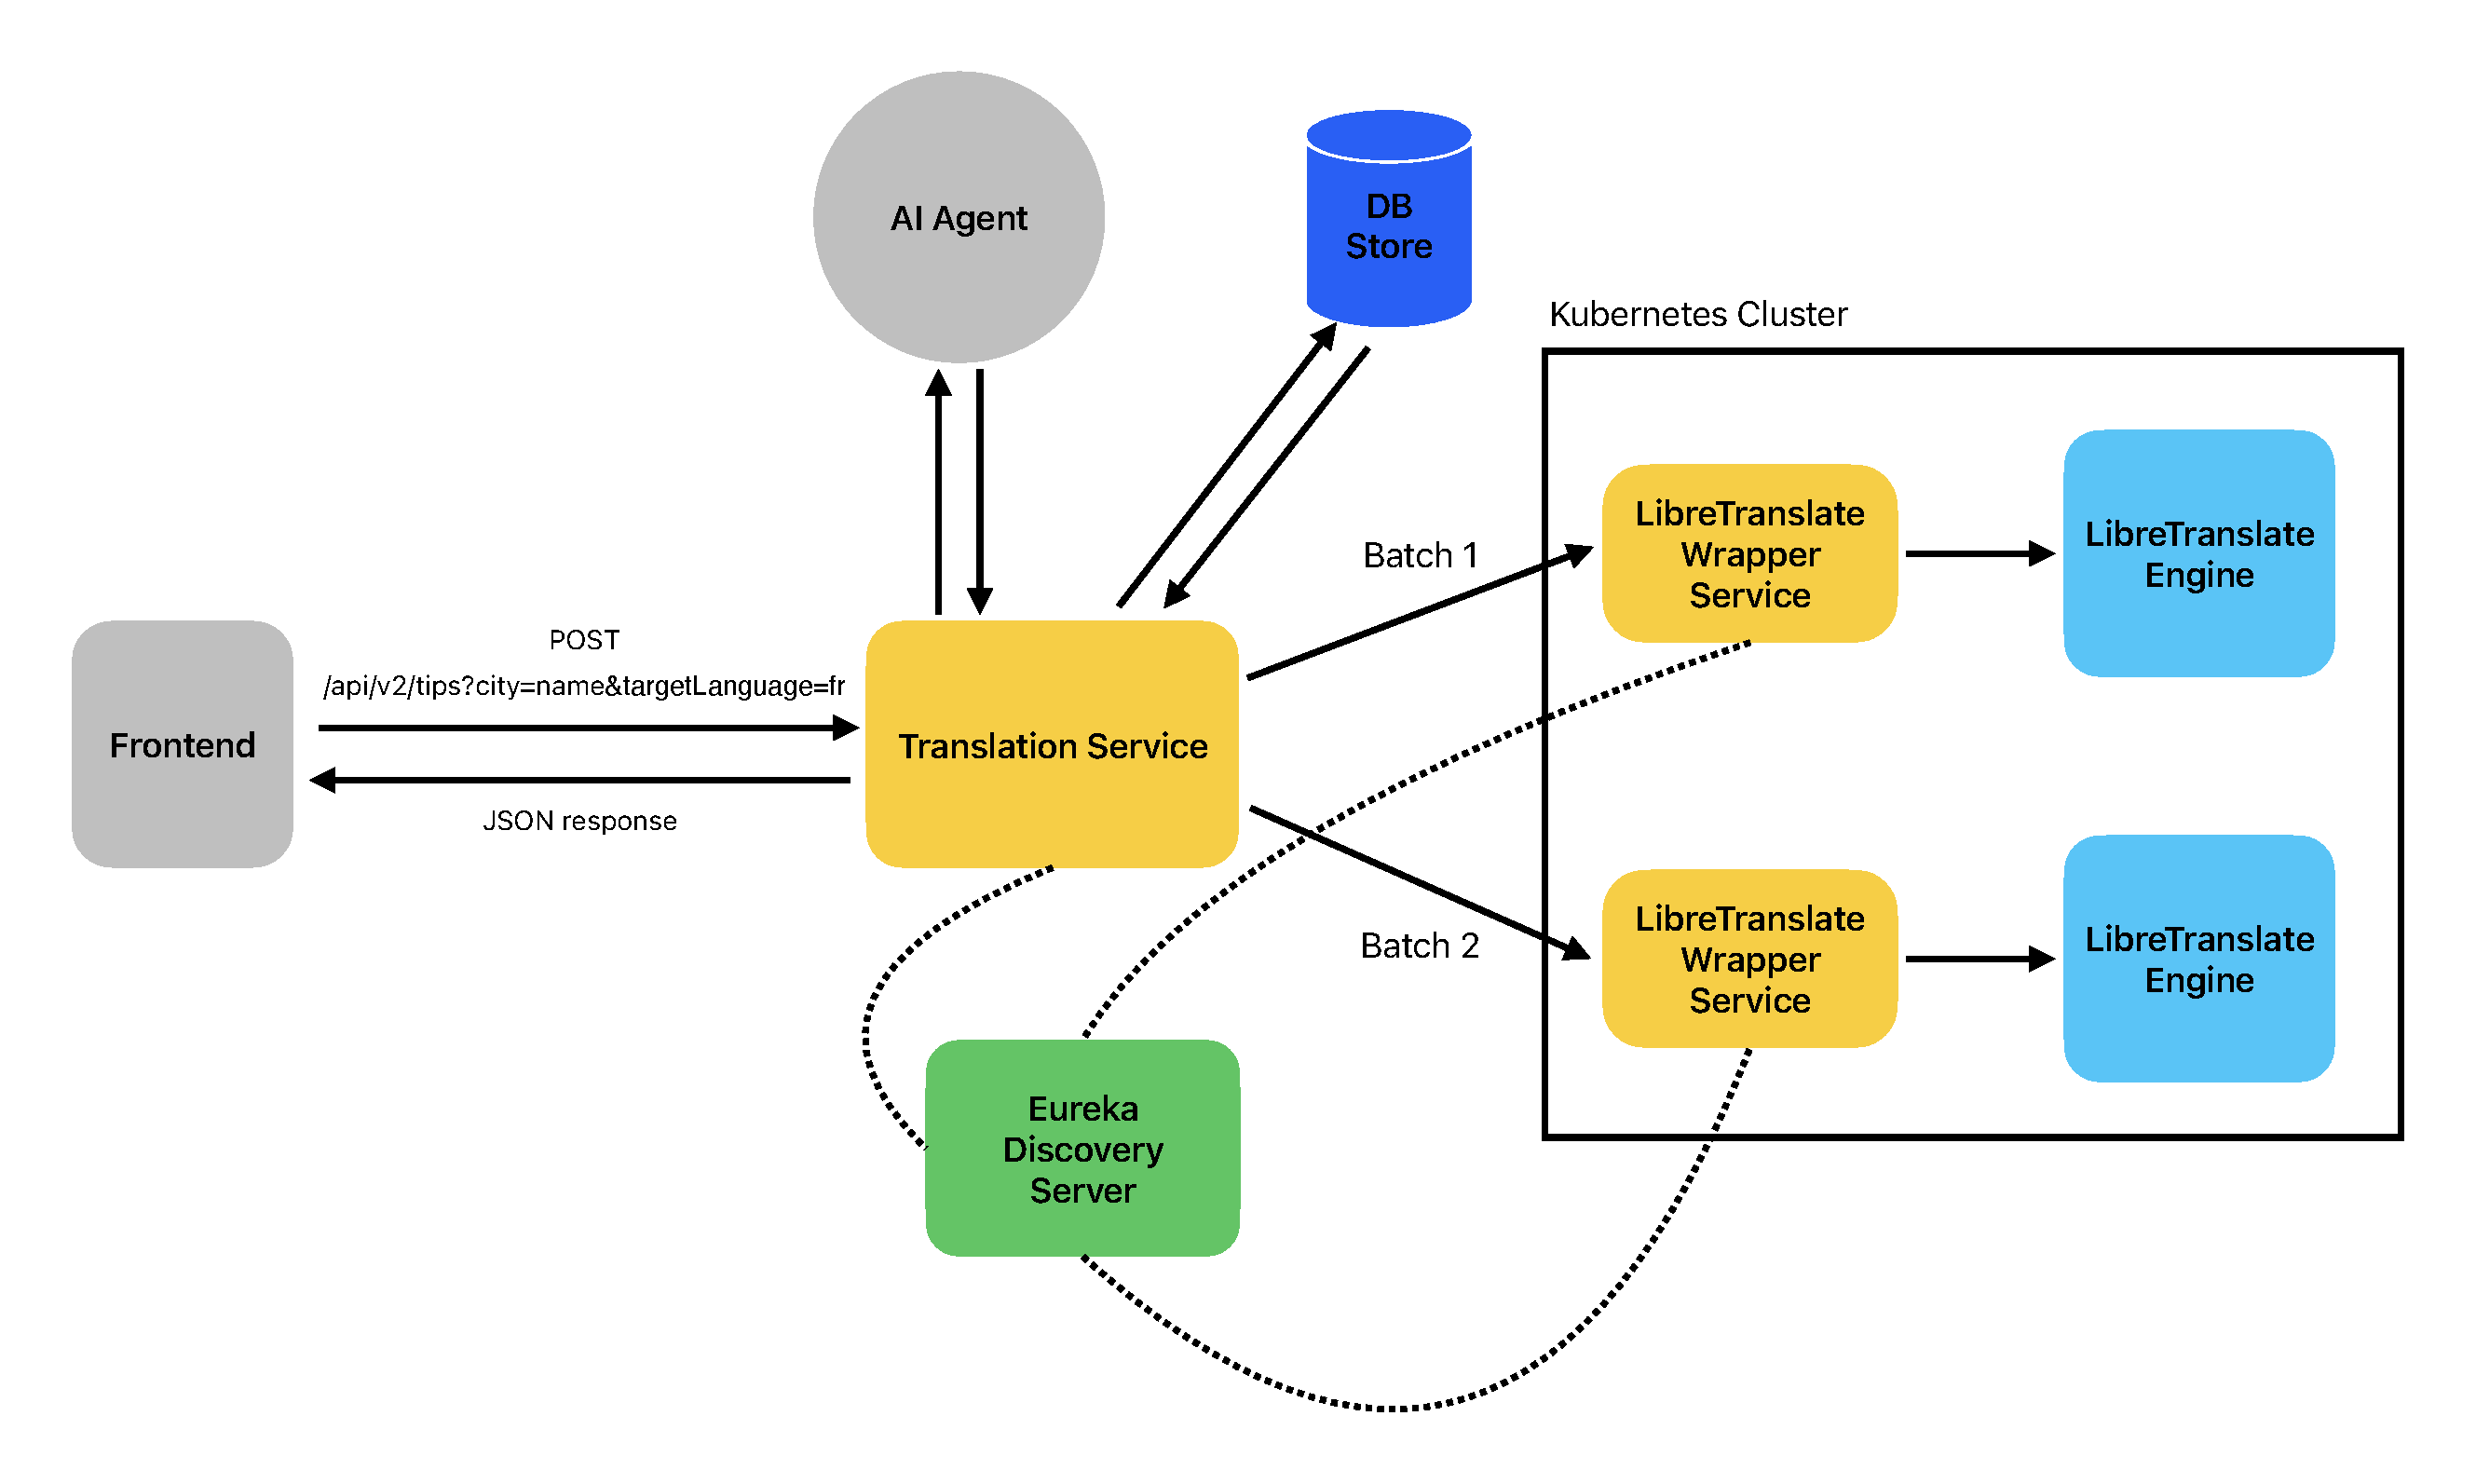
\includegraphics[width=1\linewidth]{chapter/05_implementation/backend/B_architectural_design/Backend_Iteration_4.pdf}
    \caption{Fourth iteration of backend service}
    \label{fig:backend_iteration_4}
\end{figure}